% Synthesis prompt chat UI — Ch.4 Definition~\ref{def:prompt}
% SYSTEM: left-aligned; USER messages: right-aligned (labels + bubbles)
\usetikzlibrary{positioning, shadows.blur, fit, backgrounds, calc}

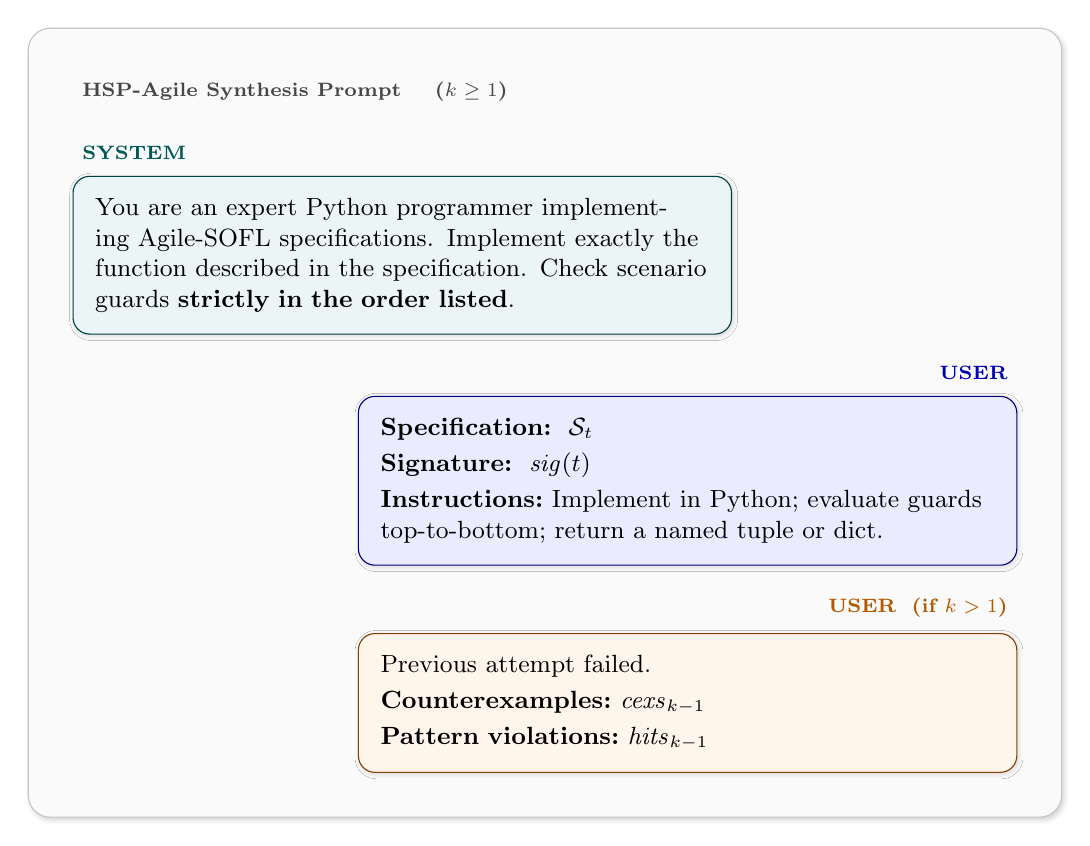
\begin{tikzpicture}[
  font=\small,
  bubble/.style={
    draw=#1!50!black, fill=#1!8, rounded corners=6pt,
    text width=7.8cm, align=left, inner sep=8pt,
    blur shadow={shadow xshift=0.5pt, shadow yshift=-0.6pt,
                 shadow blur steps=3, shadow opacity=15}
  },
  roleL/.style={font=\scriptsize\bfseries, text=#1!70!black, anchor=north west},
  roleR/.style={font=\scriptsize\bfseries, text=#1!70!black, anchor=north east}
]

\coordinate (chatL) at (0, 0);
\coordinate (chatR) at (12, 0);

% ── Title ────────────────────────────────────────────────────────────────────
\node[font=\scriptsize\bfseries, text=gray!55!black, anchor=north west] (title)
  at (chatL) {HSP-Agile Synthesis Prompt \quad ($k \ge 1$)};

% ── 1. SYSTEM (left) ─────────────────────────────────────────────────────────
\node[roleL=teal] (syslab) at ([yshift=-0.32cm]title.south west) {SYSTEM};

\node[bubble=teal, anchor=north west] (sys)
  at ([yshift=-0.08cm]syslab.south west) {%
  You are an expert Python programmer implementing Agile-SOFL
  specifications. Implement exactly the function described in the
  specification. Check scenario guards \textbf{strictly in the order listed}.};

% ── 2. USER (right) ──────────────────────────────────────────────────────────
\node[roleR=blue] (usrlab)
  at ([yshift=-0.28cm]sys.south -| chatR) {USER};

\node[bubble=blue, anchor=north east] (usr)
  at ([yshift=-0.08cm]usrlab.south east) {%
  \textbf{Specification:}\ \ $\mathcal{S}_t$\\[2pt]
  \textbf{Signature:}\ \ $\mathit{sig}(t)$\\[2pt]
  \textbf{Instructions:}\ Implement in Python; evaluate guards top-to-bottom;
  return a named tuple or dict.};

% ── 3. USER repair extension (right; same bubble chrome, orange accent) ──────
\node[roleR=orange] (replab)
  at ([yshift=-0.28cm]usr.south -| chatR) {USER \;{\scriptsize(if $k>1$)}};

\node[bubble=orange, anchor=north east] (repair)
  at ([yshift=-0.08cm]replab.south east) {%
  Previous attempt failed.\\[2pt]
  \textbf{Counterexamples:}\ $\mathit{cexs}_{k-1}$\\[2pt]
  \textbf{Pattern violations:}\ $\mathit{hits}_{k-1}$};

% ── Outer frame ──────────────────────────────────────────────────────────────
\begin{scope}[on background layer]
  \node[
    fit=(title)(syslab)(sys)(usrlab)(usr)(replab)(repair),
    draw=gray!45, fill=gray!4, rounded corners=8pt,
    inner sep=16pt,
    blur shadow={shadow xshift=0.8pt, shadow yshift=-1pt,
                 shadow blur steps=5, shadow opacity=20}
  ] {};
\end{scope}

\end{tikzpicture}
